\section{Software Development Approach}

Software Development Approaches have been in place since the 1970s. They range from rigid, long-term methods such as \emph{Waterfall}. through to experimental and risky approaches like \emph{Extreme Programming}. Factors such as team size, business goals and clients all contribute to choosing the correct approach.

To identify the correct software development process to use we must first decide on some attributes of the project of which we can compare across various approaches. The following have been derived from the project ideas and plan:

\begin{enumerate}
  \item \textbf{Team Size} -
    Most of the development throughout this project will be done by one person. This removes the need for large-scale approaches such as \emph{Waterfall} and \emph{Spiral} and instead opens up the possibility of a faster, looser process such as \emph{Agile}.
  \item \textbf{Client Interaction} - 
    If the project idea is accepted we will be allowed to work very closely with a representive from Atos. This means our development approach needs to incorporate this throughout the entire lifecycle, making methodologies such as \emph{Waterfall} less relevant since they do not encourage client interaction during the development stage.
  \item \textbf{Timeline} - 
    The entire development and testing cycle for the project is only a few months, so whatever approach is chosen needs to be dynamic and allow for quick iterations without the need to go through the entire process again. This requirement makes approaches such as \emph{Incremental Development} inappropriate because they add in repeated requirements analysis and architecture design steps that may not be necessary.
  \item \textbf{Deliverable} -
    The client is expecting a working prototype to be delivered at the end of the project. The technology must be built to a satisfactory standard, but does not need to be production-ready nor be immaculately written. This allows for the testing, integration and implementation steps in the software development approach to be removed as a priority and opens up the possibility of using less formal approaches such as \emph{Prototyping} and \emph{Extreme Programming}.
\end{enumerate}
These requirements narrow the scope down to three relevant approaches:

\begin{itemize}
  \item \textbf{Agile} - 
    Agile development promotes principles such as continous improvement, early delivery, adaptive planning and evolutionary development. It breaks tasks down into small increments, with the goal of each increment being a new release. There is a big focus on quick communication and easy feedback, normally achieved by daily standup meetings and regular planning sessions. Whilst the communication principles would be useful for this project, the approach also tends to have a relience on multiple teams tackling the project which is not relevant.
  \item \textbf{Prototyping} - 
    Software prototyping is perfect for projects where a production-ready deliverable is not required. Each iteration of the project has no requirement to fully work or meet the users' requirements. Instead, the software goes through an iterative modification process until user acceptance is met or the prototype is discarded.
    The downfall of prototyping is that it is a very relaxed approach. Client interaction is suggested, not enforced, and often the developers may lose sight of the completed project by getting too involved in a limited prototype which ultimately is only a partial representation of the desired product.
  \item \textbf{Rapid Application Development (RAD)} - 
    RAD is used to describe alternatives to the \emph{Waterfall} approach that focus on iterative development rather than formal, structured planning cycles. The most common definition of RAD, created by James Martin, involves an initial requirements planning stage followed by an interative construction and user feedback stage.

    \begin{minipage}{\linewidth}
      \centering
      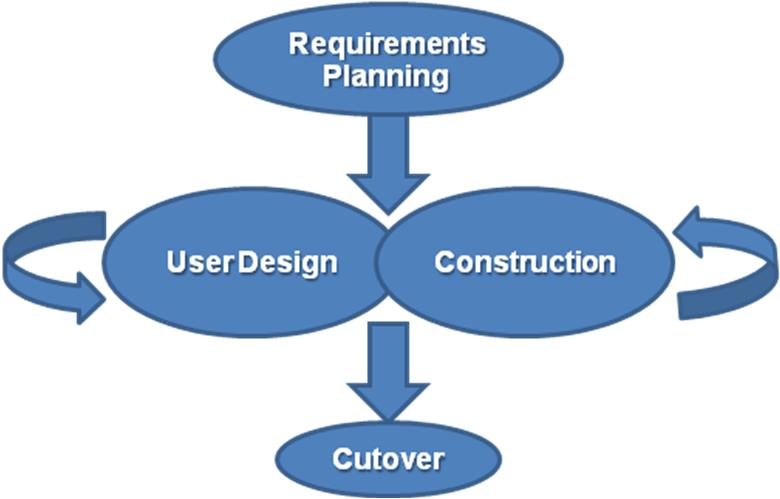
\includegraphics[width=0.5\textwidth]{./img/rad-model.jpg}
      \captionof{figure}{Phases in the James Martin approach to RAD}
    \end{minipage}

    This fits in nicely with the four project attributes we defined above:
    \begin{enumerate}
      \item \textbf{Team Size} - 
        RAD imposes no requirements on number, size or iteractions of teams.
      \item \textbf{Client Interaction} - 
        The UserDesign stage requires development to go hand in hand with client feedback and testing.
      \item \textbf{Timeline}
        There is no restriction on the length of the UserDesign/Construction process in RAD, allowing for the development cycle to last as long as possible before the deadline is reached without having to estimate iterations during early planning stages.
      \item \textbf{Deliverable}
        There are no formal requirements for repetitive testing and quality control. This can be implemented independently from the software development approach, allowing for testing to be suited to the individual project.
    \end{enumerate}
\end{itemize}
The analysis above clearly identifies \emph{Rapid Application Development} as the most appropriate software development approach for this project.